\section{Product overview}

The aim of this product is to serve as a simulator for a Bowling Alley. We want to be able to simulate players coming in groups ("party") to the alley and being assigned a lane to bowl on. If there's no lane yet, then they wait in a queue. While bowling, they proceed frame by frame, being able to see pins falling on a pinsettter as well as see their detailed scorecard on a scoresheet.

Once the party is done bowling, they can play another game if they wish to. Otherwise, they can take a printout of their performance and leave the alley. There are three lanes in the alley, each allowing a party to have six players.

In the refactored product, we were also asked to implement additional features, expanding the scope of this simulator. Namely, we now allow a party to pause their game in between and leave the alley. Later, they can resume their unfinished game.

We now also support ad-hoc queries on the user data. Each player can view their best and worst score statistics, as well as their career top five scores.

\subsection{Product screenshots}

\begin{figure}[H]
    \centering
    \begin{subfigure}{\textwidth}
        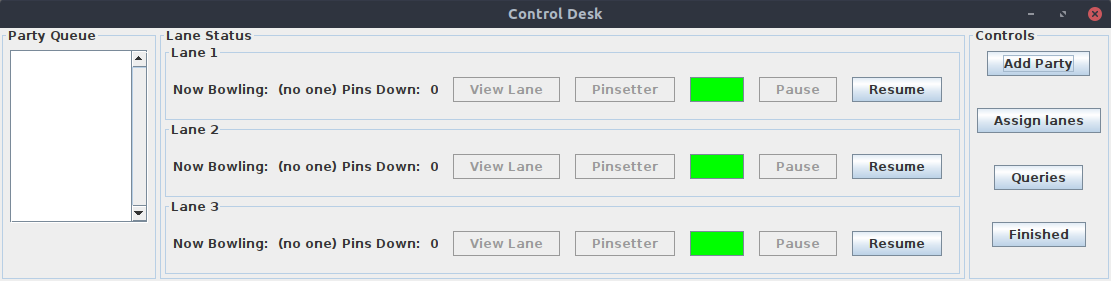
\includegraphics[width = \textwidth]{img/controldesk.png}
        \caption{The main control desk, where we can create parties, assign them to lanes, or ask for ad-hoc queries.}
    \end{subfigure}
    \begin{subfigure}{\textwidth}
        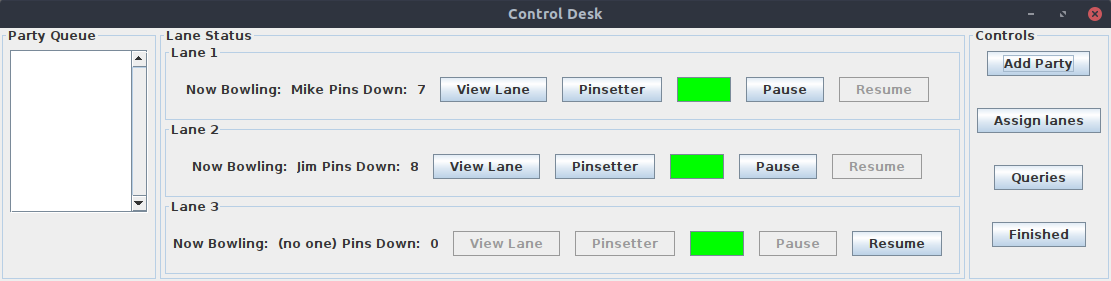
\includegraphics[width = \textwidth]{img/laneRunning.png}
        \caption{When a party is playing on the first two lanes.}
    \end{subfigure}
    \caption{Control Desk}
\end{figure}

\begin{figure}[H]
    \centering
    \begin{subfigure}{\textwidth}
        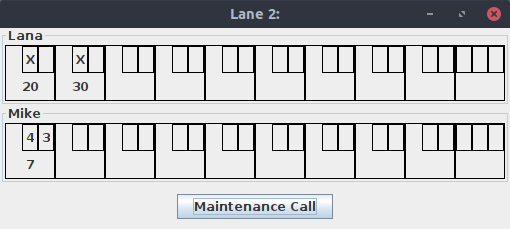
\includegraphics[width = \textwidth]{img/lanestatus.png}
        \caption{Dynamically updated scoresheet of players in a party as they bowl.}
    \end{subfigure}
    \begin{subfigure}{\textwidth}
        \centering
        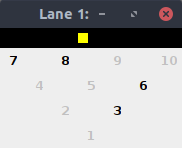
\includegraphics[width = 0.4\textwidth]{img/pinsetter.png}
        \caption{Dynamically updated pinsetter, shows pins standing as dark black, and fallen as light grey}
    \end{subfigure}
    \caption{Dynamic lane view elements}
\end{figure}

\begin{figure}[H]
    \centering
    \begin{subfigure}{\textwidth}
        \centering
        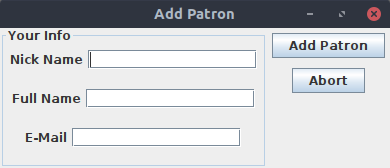
\includegraphics[width = 0.8\textwidth]{img/addpatron.png}
        \caption{Add patron modal}
    \end{subfigure}
    \begin{subfigure}{\textwidth}
        \centering
        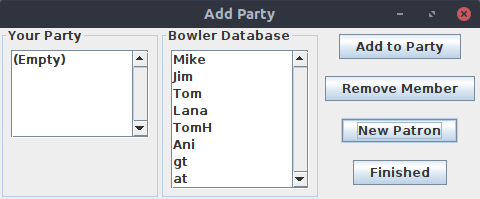
\includegraphics[width = 0.8\textwidth]{img/addparty.png}
        \caption{Add party modal}
    \end{subfigure}
    \caption{The data update modals}
\end{figure}

\begin{figure}[H]
    \centering
    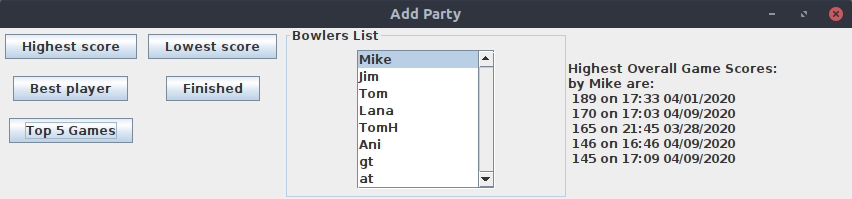
\includegraphics[width = \textwidth]{img/queries.png}
    \caption{Ad-hoc queries modal, dynamically fetches statistics from the storage}
\end{figure}

\subsection{Our dedication to software engineering principles}

Throughout our refactoring, we have consistently upholded major principles of software design. The first is obviously \textbf{DRY} - Don't Repeat Yourself. This is a common principle, wherein we make sure that the same functionality is not duplicated in more than one place. In our project, we have ensured that even the simplest of logics, like checking whether a strike occurred or not (\code{pinsDown == 10}) has been carefully placed in a dedicated method so as to not duplicate it across mutliple places.

Another principle we stuck to was \textbf{Single Responsibility principle}: which states that every class should be responsible for exactly one purpose. Note that this was the hardest to sustain, since the original codebase had a God class (Lane.java) by itself.

\textbf{Law of Demeter} was another arena we conquered. We ensured that our classes are kept independent of each other, that connections between different classes are minimized (\textbf{coupling}), and that related classes are kept together (\textbf{cohesion}).

We have also extensively used \textbf{inheritance} wherever required to convey the semantic logic of our classes. For example, \code{BowlerInfo} acts as a base class for \code{Bowler}. The sole responsibility of BowlerInfo is to keep track of metadata of a Bowler, whereas the sole role of a Bowler is to be able to roll balls down a lane. We then implemented \code{ScorableBowler} which inherits from Bowler, and also adds the ability to keep track of scores across games. This chain of inheritance ensures that our classes have cohesive usage of attributes as well as reusability throughout.